\documentclass[border=10pt]{standalone}
\usepackage[svgnames]{xcolor}
\usepackage{amsmath}
\usepackage{pgfplots}
\pgfplotsset{compat=newest}
\usepackage[sfdefault]{FiraSans}
\usepackage{FiraMono}
\renewcommand*\familydefault{\sfdefault}
\begin{document}
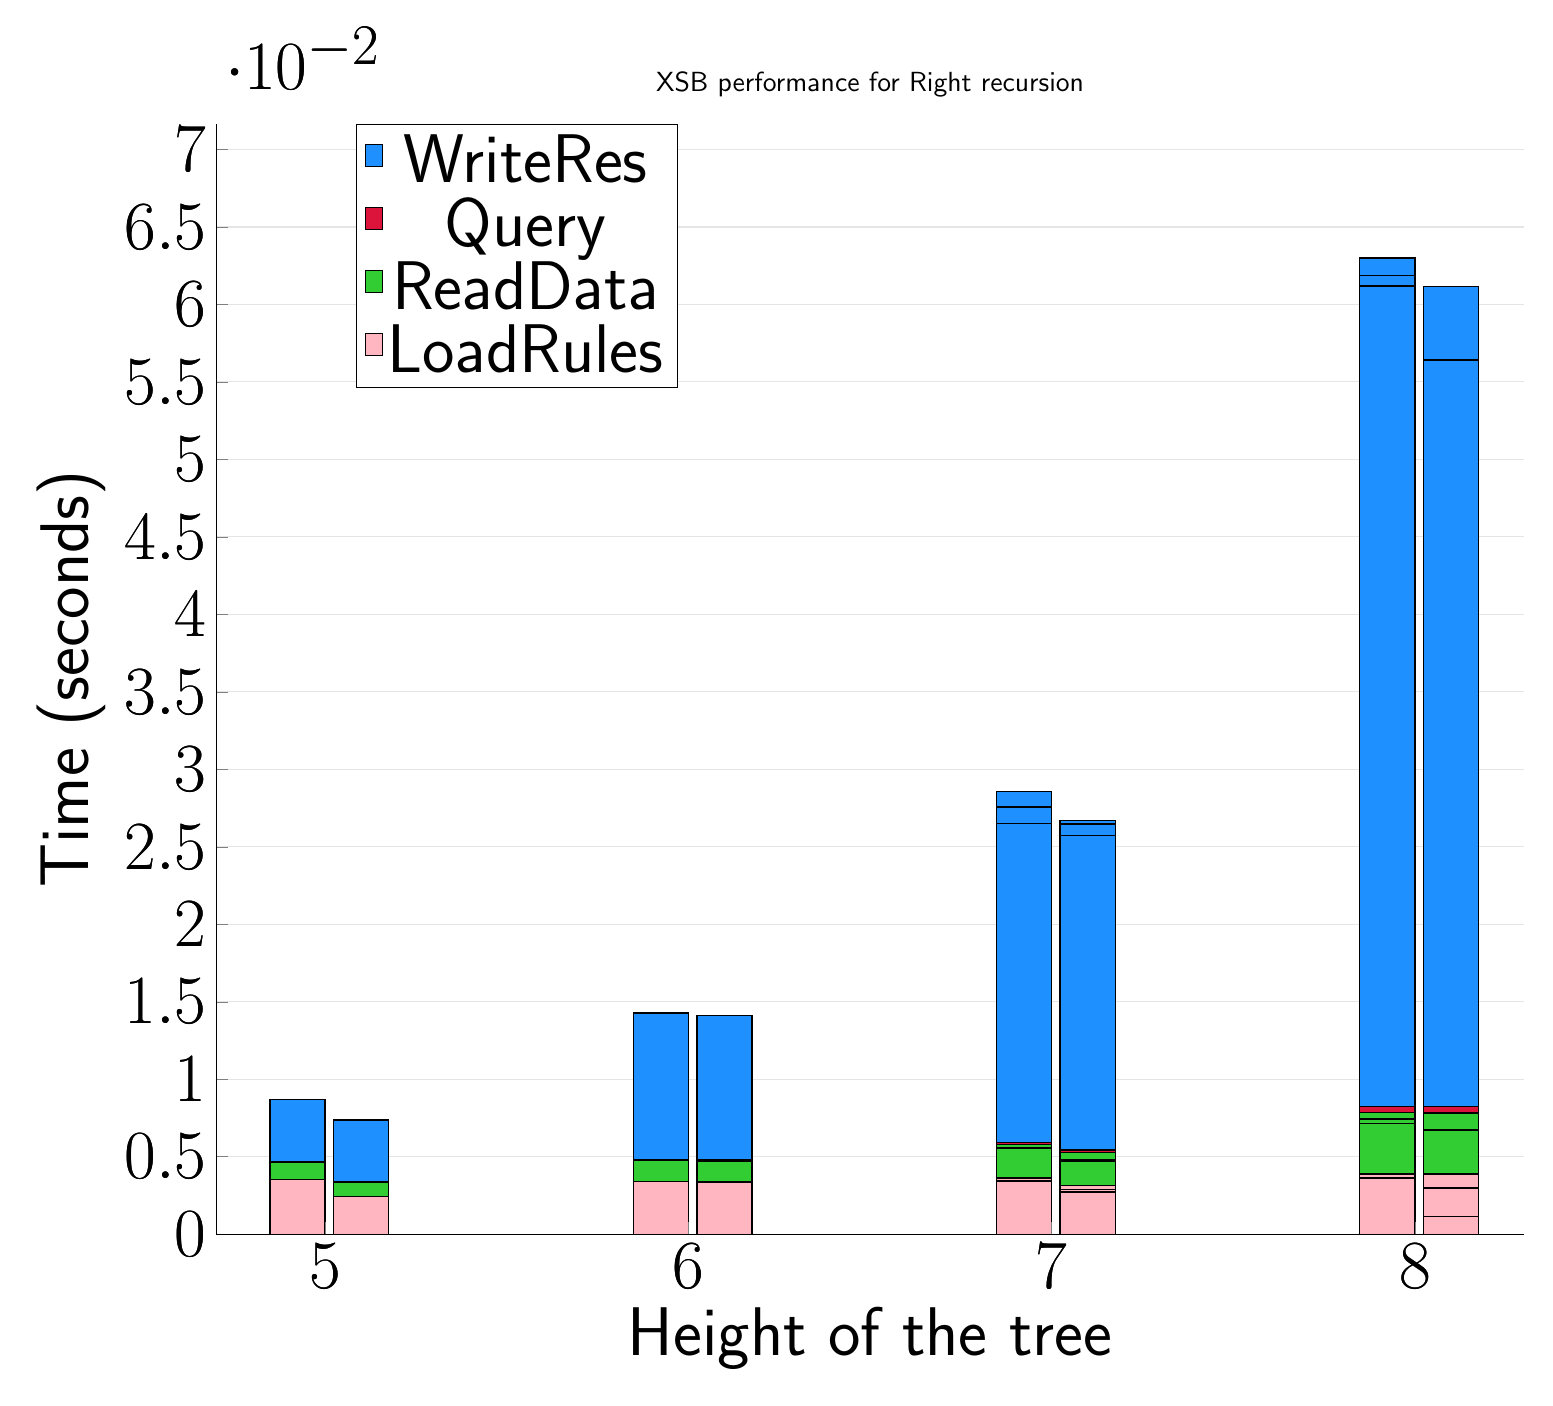
\begin{tikzpicture}
\begin{axis}[
   ybar stacked,
   title={XSB performance for Right recursion},
   bar shift=-10pt,
   width=1.5\textwidth,
   bar width=0.7cm,
   ymajorgrids, tick align=inside,
   major grid style={draw=gray!20},
   xtick=data,
   ymin=0, ymax=0.07167722702026368,
   axis x line*=bottom,
   axis y line*=left,
   enlarge x limits=0.1,
   legend style={
       at={(0.23, 1)},
       anchor=north,
       legend columns=1,
       font=\Huge,
   },
   ylabel={Time (seconds)},
   xlabel={Height of the tree},
   label style={font=\Huge},
   tick label style={font=\Huge},
]
\addlegendimage{fill=DodgerBlue, draw=black, line width=0.2pt}
\addlegendentry{WriteRes}
\addlegendimage{fill=Crimson, draw=black, line width=0.2pt}
\addlegendentry{Query}
\addlegendimage{fill=LimeGreen, draw=black, line width=0.2pt}
\addlegendentry{ReadData}
\addlegendimage{fill=LightPink, draw=black, line width=0.2pt}
\addlegendentry{LoadRules}
\addplot +[fill=LightPink, draw=black, line width=0.5pt] coordinates {
    (5, 0.00351460774739583)
    (6, 0.0033853054046630864)
    (7, 0.0034068425496419264)
    (7, 0.0036189556121826168)
    (7, 0.0034793217976887996)
    (8, 0.003663937250773113)
    (8, 0.0038970311482747367)
    (8, 0.0035927295684814436)
};
\addplot +[fill=LimeGreen, draw=black, line width=0.5pt] coordinates {
    (5, 0.0011212825775146508)
    (6, 0.0013573169708251964)
    (7, 0.00215609868367513)
    (7, 0.002153714497884117)
    (7, 0.00206502278645833)
    (8, 0.003776073455810547)
    (8, 0.003940264383951823)
    (8, 0.003563404083251953)
};
\addplot +[fill=Crimson, draw=black, line width=0.5pt] coordinates {
    (5, 4.474322001139323e-05)
    (6, 7.168451944986977e-05)
    (7, 0.00015926361083984367)
    (7, 0.00015759468078613268)
    (7, 0.00017491976420084635)
    (8, 0.00039299329121907567)
    (8, 0.00039998690287272126)
    (8, 0.0003482500712076823)
};
\addplot +[fill=DodgerBlue, draw=black, line width=0.5pt] coordinates {
    (5, 0.00399438540140788)
    (6, 0.009458621342976883)
    (7, 0.02185106277465822)
    (7, 0.022634506225585934)
    (7, 0.020776033401489254)
    (8, 0.0540417035420736)
    (8, 0.05295062065124515)
    (8, 0.05548381805419922)
};
\end{axis}
\begin{axis}[
   ybar stacked,
   bar shift=13pt,
   width=1.5\textwidth,
   bar width=0.7cm,
   ymajorgrids, tick align=inside,
   major grid style={draw=none},
   xtick=data,
   ymin=0, ymax=0.07167722702026368,
   axis x line*=none,
   axis y line*=none,
   enlarge x limits=0.1,
   label style={font=\Huge},
   tick label style={font=\Huge},
]
\addplot +[fill=LightPink, draw=black, line width=0.5pt] coordinates {
    (5, 0.0024403333333333334)
    (6, 0.0033583333333333334)
    (7, 0.0028820000000000004)
    (7, 0.003137000000000003)
    (7, 0.002713)
    (8, 0.0029806666666666666)
    (8, 0.003885000000000003)
    (8, 0.00115)
};
\addplot +[fill=LimeGreen, draw=black, line width=0.5pt] coordinates {
    (5, 0.0008856666666666657)
    (6, 0.0013579999999999998)
    (7, 0.0018166666666666635)
    (7, 0.002130333333333333)
    (7, 0.0020650000000000004)
    (8, 0.0037476666666666665)
    (8, 0.003941)
    (8, 0.0010783333333333333)
};
\addplot +[fill=Crimson, draw=black, line width=0.5pt] coordinates {
    (5, 3.5333333333333966e-05)
    (6, 7.133333333333067e-05)
    (7, 0.00013533333333333103)
    (7, 0.00015733333333333536)
    (7, 0.00017466666666666433)
    (8, 0.000392666666666666)
    (8, 0.0004003333333333313)
    (8, 0.00010599999999999966)
};
\addplot +[fill=DodgerBlue, draw=black, line width=0.5pt] coordinates {
    (5, 0.003999333333333333)
    (6, 0.009337333333333336)
    (7, 0.02185266666666667)
    (7, 0.02105)
    (7, 0.020775000000000002)
    (8, 0.05402766666666667)
    (8, 0.05292933333333333)
    (8, 0.054073)
};
\end{axis}
\end{tikzpicture}

\end{document}
